\documentclass[UTF8]{ctexart}

\usepackage{amsmath}
\usepackage{cases}
\usepackage{cite}
\usepackage{graphicx}
\usepackage[margin=1in]{geometry}
\usepackage{fancyhdr}
\usepackage{float}
\usepackage{listings}
\usepackage{ctex}
\usepackage{xcolor}
\usepackage{fontspec}
\usepackage{titling}
\pagestyle{fancy}
\fancyhf{}
\geometry{a4paper}

\lstset{ %代码块设置
    language = C,
    numbers=left,
    keywordstyle=\color{blue!70},
    commentstyle=\color{red!50!green!50!blue!50},
    frame=shadowbox,
    rulesepcolor=\color{red!20!green!20!blue!20},
    basicstyle=\ttfamily,
    showstringspaces=false
}
\lstset{language=C}

\title{Fashion-MNIST 图像分类实验报告}
\author{\LaTeX\ by\ 密语Smera1d0}
\date{\today}
\pagenumbering{arabic} %设置文章页码为阿拉伯数字

\begin{document}
\fancyhf{}
\fancyhead[L]{ %页眉左侧logo
    \begin{minipage}[c]{0.9\textwidth}
        
\includegraphics[height=10.5mm]{picture/logo.png}
    \end{minipage}
}
\fancyhead[C]{Fashion-MNIST 图像分类实验报告}
\fancyfoot[C]{\thepage}

\begin{titlepage}                                               %用于单人报告的封面 For single report 
    \centering
    
\includegraphics[width=0.65\textwidth]{picture/logo_text.png}   % 插入你的图片,调整文件名和路径 Insert your picture, adjust the file name and path
    \par\vspace{1.5cm}
    {\Huge \heiti Fashion-MNIST 图像分类实验报告 \par} % 标题 Title
    \vspace{1cm}
    {\Large \heiti 《计算机视觉》Assignment 1\par}              % 副标题 Subtitle
    \vspace{5cm}


    % 个人信息  Personal information
    \begin{center}
        {\Large                                                 % 这里的字号也可以用别的方式修改   The font size here can also be modified in other ways
        \makebox[4em][s]{\heiti 姓名}:\underline{\makebox[15em][c]{\heiti 董霁兴}}\\
        \makebox[4em][s]{\heiti 学号}:\underline{\makebox[15em][c]{\heiti 2024317181}}\\
        \makebox[4em][s]{\heiti 班级}:\underline{\makebox[15em][c]{\heiti 计算机技术2班}}\\
        \makebox[4em][s]{\heiti 学院}:\underline{\makebox[15em][c]{\heiti 信息科学与工程学院}}\\
        }
    \end{center}

    \vfill
    \today % 日期
\end{titlepage}


\newpage

\tableofcontents  %自动根据下文创建目录


\newpage
\section{引言}
在计算机视觉领域,图像分类任务一直是研究的重点之一。对于初入计算机视觉领域的学习者而言,进行图像分类实验是深入理解该领域核心概念和技术的重要途径。本次实验选取 Fashion-MNIST 数据集,旨在对比不同深度的卷积神经网络模型,尤其是早期的 LeNet 网络与较为先进的 ResNet 模型,以深入研究深度网络的架构设计、图像分类的关键技术以及模型训练的有效方法。同时,通过观察超参数调优对模型性能的影响,为后续在计算机视觉领域的学习和研究积累经验。

\section{实验目的}
\begin{enumerate}
\item 作为计算机视觉学习的基础实践,深入掌握深度网络的基本结构、图像分类的流程以及模型训练的关键环节,为后续在该领域的深入学习和研究奠定基础。
\item 系统对比早期经典的 LeNet 网络与先进的 ResNet(ResNet18 和 ResNet34)模型在 Fashion-MNIST 数据集上的性能差异,包括但不限于训练准确率、测试准确率、训练速度等多个指标,以全面评估不同模型的优势与不足。
\item 深入探究超参数(如学习率等)的调整对不同模型训练效果的具体影响,明确超参数调优在模型性能提升中的重要作用,掌握有效的超参数调优方法和策略。
\item 通过对实验结果的分析,总结不同模型在特定数据集下的适用性和局限性,为实际应用中模型的选择提供科学依据。
\item 培养在计算机视觉领域解决实际图像分类问题的能力,提高对复杂问题的分析和处理水平。
\end{enumerate}

\section{实验环境}
\subsection{硬件环境}
本实验使用个人笔记本电脑进行训练,i7 14650HX 处理器和 RTX 4060 Laptop 显卡的设备,CUDA版本为 12.6

\subsection{软件环境}
实验采用 Python 3.9,和 PyTorch 深度学习框架。自行实现了一些用于展示损失曲线的工具类。

\subsection{数据集}
本次实验选用的是 Fashion-MNIST 数据集。此数据集由 60,000 个训练样本和 10,000 个测试样本组成,共涵盖了十个不同的时尚类别,其中包括 T 恤、裤子、连衣裙等。该数据集具有以下显著特点:其图像皆为灰度图,尺寸统一为 28x28 像素。虽然在泛用性方面不及 ImageNet 数据集,但相较于传统的 MNIST 数据集,Fashion-MNIST 更具挑战性。同时,在 RTX 4060 Laptop 的硬件环境下,该数据集能够较快地进行训练,综合考虑各方面因素,选取 作 Fashion-MNIST 为本次实验的数据集。

\section{实验设置}
\subsection{模型架构}
\begin{enumerate}
    \item LeNet:LeNet 作为最早发布的卷积神经网络之一,由 AT\&T 贝尔实验室的研究员 Yann LeCun 于 1989 年提出并以其命名,它是计算机视觉领域的重要起步,是一个 5 层的卷积神经网络,由卷积层、池化层和全连接层组成,
    \item ResNet18:ResNet18 是一种包含 18 层的残差网络。残差网络通过引入残差块,解决了深度神经网络在训练过程中出现的梯度消失和梯度爆炸问题。相比作为起步的 LeNet,ResNet18 在性能和特征学习能力上更为高级。
    \item ResNet34:ResNet34 包含 34 层,比 ResNet18 更深。随着层数的增加,模型可以学习到更复杂的特征表示。
\end{enumerate}

\subsection{训练参数}
\begin{itemize}
    \item 批次大小:256
    \item 训练轮数:10轮
    \item 优化器:随机梯度下降(SGD)
    \item 学习率:[0.1, 0.05, 0.01]
\end{itemize}

\section{实验结果与分析}
\subsection{模型性能对比}
\begin{table}[H]
    \centering
    \begin{tabular}{|c|c|c|c|c|}
        \hline
        模型 & 学习率 & 训练准确率 & 测试准确率 & 训练速度(样本/秒) \\
        \hline
        LeNet & 0.1 & 89.4\% & 83.5\% & 50,245 \\
        LeNet & 0.05 & 88.2\% & 86.6\% & 48,436 \\
        LeNet & 0.01 & 83.0\% & 82.1\% & 46,412 \\
        \hline
        ResNet18 & 0.1 & 95.4\% & 81.2\% & 19,705 \\
        ResNet18 & 0.05 & 96.2\% & 89.2\% & 19,990 \\
        ResNet18 & 0.01 & 97.0\% & 87.6\% & 20,480 \\
        \hline
        ResNet34 & 0.1 & 94.2\% & 84.0\% & 11,838 \\
        ResNet34 & 0.05 & 94.9\% & 88.4\% & 12,002 \\
        ResNet34 & 0.01 & 95.4\% & 87.3\% & 11,866 \\
        \hline
    \end{tabular}
    \caption{不同模型在不同学习率下的性能对比}
\end{table}

\subsection{实验分析}
\subsubsection{学习率影响}
\begin{itemize}
    \item 对于所有模型,学习率为 0.05 时表现最佳,在训练和测试性能间取得了良好平衡。
    \item 较高的学习率(0.1)导致模型训练不稳定,特别是 ResNet 系列模型。
    \item 较低的学习率(0.01)虽然训练准确率高,但泛化性能略有下降。
\end{itemize}

\subsubsection{模型复杂度与性能}
\begin{itemize}
    \item LeNet 虽然结构简单,但在合适的学习率(0.05)下仍能达到 86.6\%的测试准确率。
    \item ResNet18 在学习率为 0.05 时取得最佳效果,测试准确率达 89.2\%。
    \item ResNet34 虽然层数更深,但性能提升有限,说明该数据集可能不需要过于复杂的模型。
\end{itemize}

\subsubsection{计算效率}
\begin{itemize}
    \item LeNet 由于结构简单,训练速度最快(约 50,000 样本/秒)。
    \item ResNet18 的训练速度约为 LeNet 的 40\%。
    \item ResNet34 训练速度进一步降低至约 12,000 样本/秒。
\end{itemize}

\section{LeNet 和 ResNet 差异及优化}
\subsection{LeNet 与 ResNet 的差异}
\subsubsection{网络层数}
\begin{enumerate}
    \item LeNet 是一个经典的 5 层卷积神经网络,相对较为简单。
    \item ResNet18 包含 18 层,ResNet34 则有 34 层,明显比 LeNet 的层数多得多。随着网络层数的增加,ResNet 能够学习到更复杂的特征表示,对图像的理解能力更强。
\end{enumerate}

\subsubsection{架构设计}
\begin{enumerate}
    \item LeNet 主要由卷积层、池化层和全连接层组成。其设计简洁,适用于处理小规模数据集和简单的图像分类任务。
    \item ResNet 引入了残差连接,这是其与 LeNet 最显著的差异之一。残差连接通过将输入直接加到输出上,使得网络可以更容易地学习恒等映射,从而缓解了深度神经网络中的梯度消失问题。这种设计使得 ResNet 可以更深,同时保持较好的性能。
    \begin{figure}[H]
        \centering
        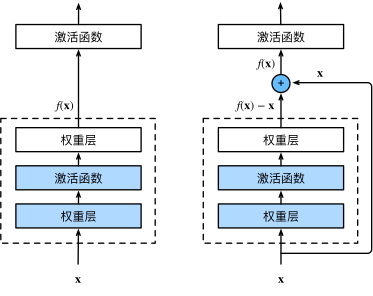
\includegraphics[width=0.4\textwidth]{picture/residual-block.png}
        \caption{残差块结构示意图}
    \end{figure}
\end{enumerate}
\subsubsection{模块结构}
\begin{enumerate}
    \item ResNet 由多个残差块组成,每个残差块包含卷积层、批归一化层和激活函数层。这种模块结构使得 ResNet 可以更加灵活地调整网络的深度和宽度,同时提高了模型的泛化能力。
    \item LeNet 没有这种模块化的设计,其结构相对固定。
\end{enumerate}
\subsubsection{性能表现}
\begin{enumerate}
    \item 在 Fashion-MNIST 数据集上,ResNet18 和 ResNet34 的性能总体上优于 LeNet。ResNet 能够取得更高的测试准确率,说明其在图像分类任务中具有更强的表达能力。
    \item LeNet 虽然结构简单,但在合适的超参数下仍能取得一定的性能。对于资源受限的情况或简单的数据集,LeNet 可能是一个更合适的选择。
\end{enumerate}

\subsection{ResNet 带来的优化}
\begin{enumerate}
    \item \textbf{缓解梯度消失问题}:深度神经网络在训练过程中常常会遇到梯度消失问题,随着网络层数的增加,梯度在反向传播过程中会逐渐减小,导致底层的网络层难以更新参数。ResNet 的残差连接有效地缓解了这个问题,使得网络可以更深,从而能够学习到更复杂的特征表示。
    \item \textbf{提高性能}:通过引入残差连接和模块化的设计,ResNet 在图像分类任务中的性能得到了显著提升。在 Fashion-MNIST 数据集上,ResNet18 和 ResNet34 的测试准确率明显高于 LeNet,证明了 ResNet 在复杂图像分类任务中的优势。
    \item \textbf{增强泛化能力}:ResNet 的模块结构和残差连接的设计提高了模型的泛化能力。在不同的学习率下,ResNet 的性能波动相对较小,说明它对学习率的变化具有一定的鲁棒性。此外,ResNet 还可以通过添加 Dropout 等正则化技术进一步提高模型的泛化能力。
    \item \textbf{可扩展性}:ResNet 的模块化设计使得它可以更加容易地扩展到更深的网络结构,同时保持较好的性能。这使得 ResNet 在处理更复杂的图像分类任务时具有更大的优势,可以根据具体的任务需求调整网络的深度和宽度。
\end{enumerate}

\section{实验结论}

本次实验通过对 Fashion-MNIST 数据集的图像分类任务进行研究,对比了早期的 LeNet 网络与先进的 ResNet 模型,同时探究了超参数调优对模型性能的影响。
\begin{enumerate}
    \item 从模型性能方面来看,ResNet18 和 ResNet34 在测试准确率上总体优于 LeNet,这体现了先进的残差网络在特征学习能力上的优势。然而,LeNet 在合适的超参数下仍能取得不错的性能,说明对于特定的简单数据集,早期的经典模型也有其应用价值。
    \item 关于超参数调优,不同的学习率对各个模型的影响不同。较高的学习率(如 0.1)会导致模型训练不稳定,特别是对于 ResNet 系列模型而言,可能会使模型在更新参数时跳过最优解,从而难以收敛。而较低的学习率(如 0.01)虽然在训练过程中能使准确率较高,但会使模型的泛化性能略有下降,可能会陷入局部最优解,难以在测试集上取得良好的表现。这充分表明在模型训练过程中,合理选择超参数至关重要,它直接影响着模型的性能和收敛情况。对于此次任务下的模型,学习率为 0.05 时在训练和测试性能间取得了较好的平衡。
    \item 在计算效率方面,LeNet 由于结构简单,训练速度最快。随着 ResNet 模型层数的增加,训练速度逐渐降低。在实际应用中,需要根据具体的资源和性能需求来选择合适的模型。
    \item 通过本次实验,作为计算机视觉学习的起步,深入理解了深度网络的架构设计、图像分类的流程以及模型训练的关键环节。同时,也明确了不同模型在特定数据集下的适用性和局限性,为今后在计算机视觉领域的学习和实践提供了宝贵的经验。
    \item 对于未来的研究方向,可以进一步探索更多的超参数组合,尝试不同的优化器,以及实现模型集成等方法来进一步提升图像分类性能。同时,也可以将本次实验的方法应用到其他数据集上,进一步
\end{enumerate}

\newpage
\section{附录:训练结果}
\subsection{LeNet 在不同学习率下的训练结果}
\begin{center}
\begin{minipage}{\textwidth}
\begin{figure}[H]
    \centering
    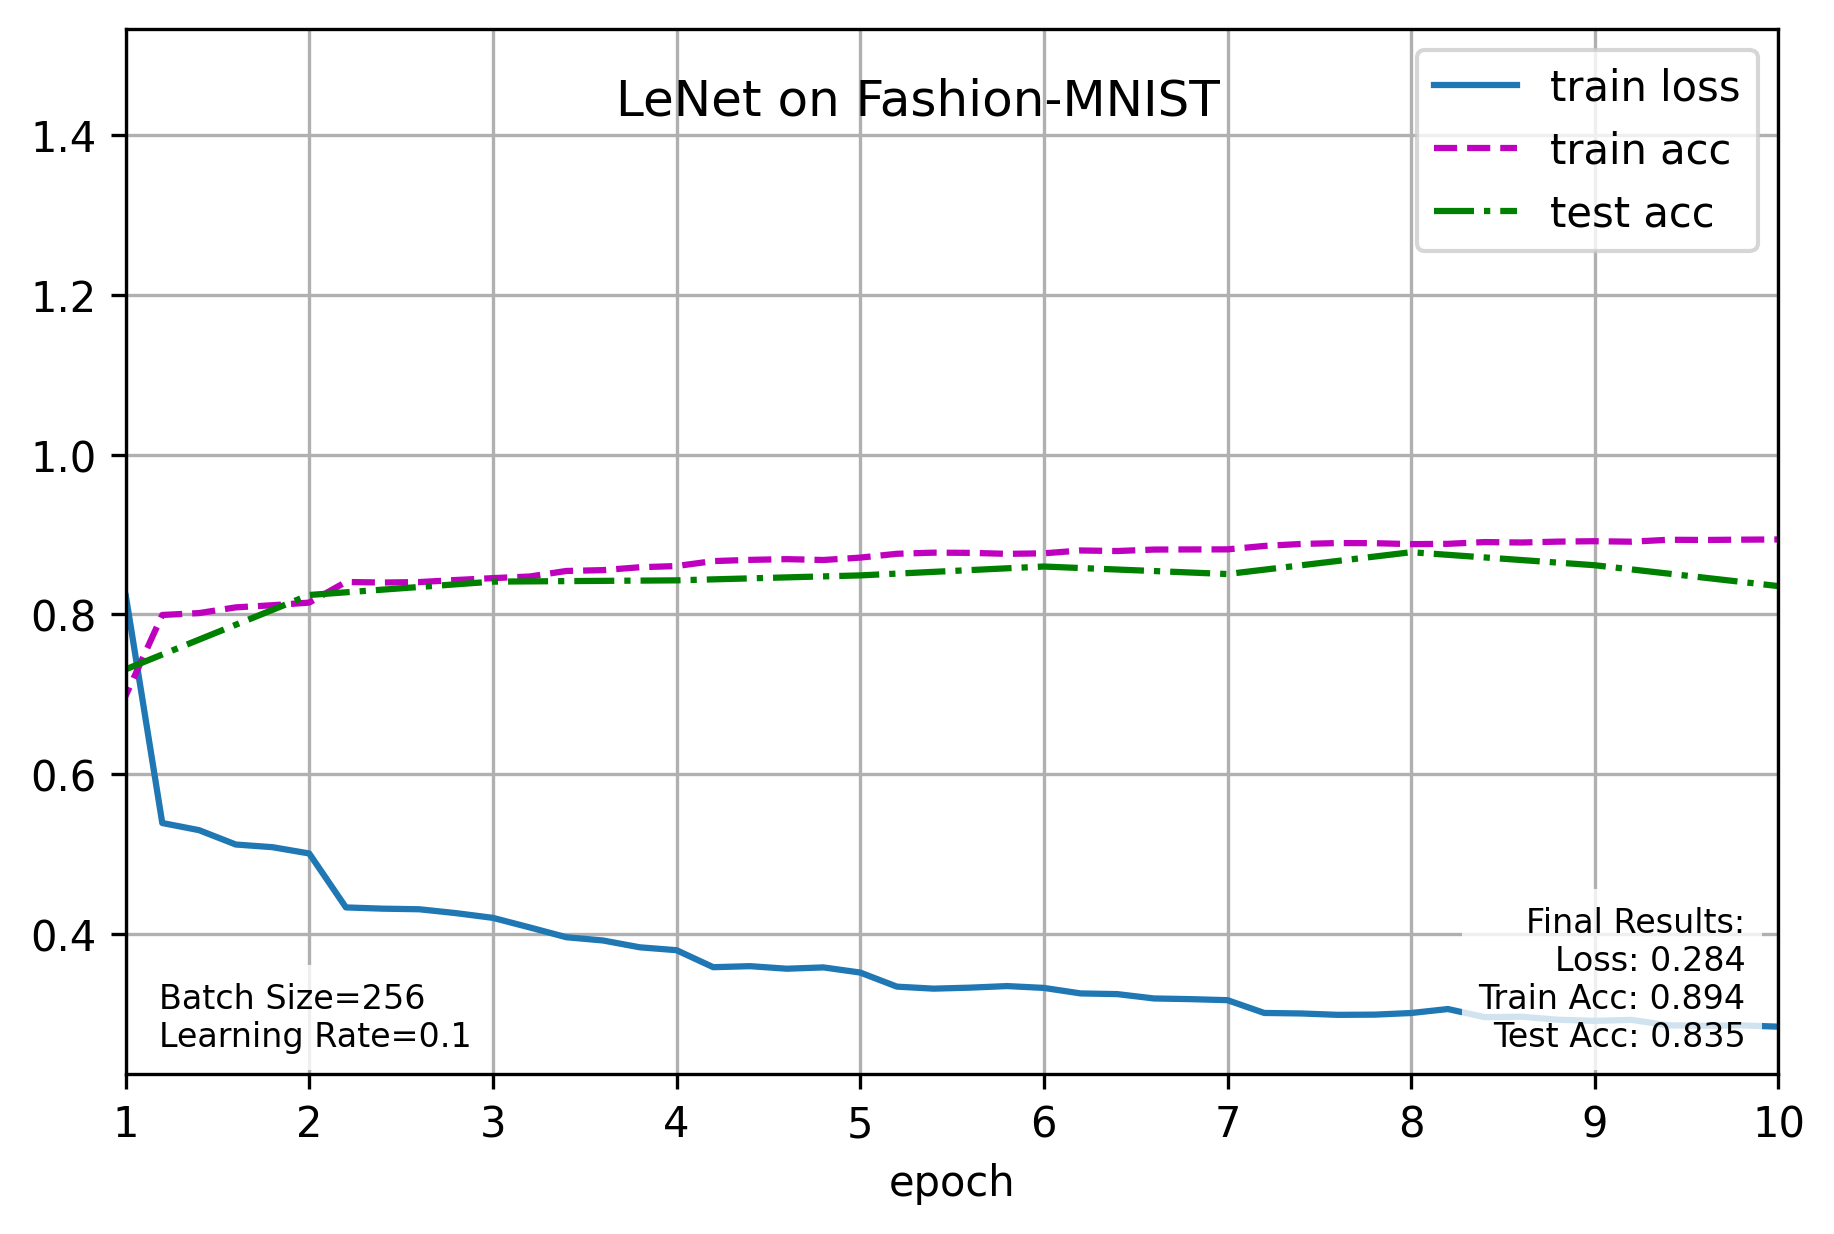
\includegraphics[width=0.6\textwidth]{picture/lenet_on_fashion-mnist_bs256_lr0.1_20241110_221026.png}
    \caption{LeNet 使用 0.1 学习率训练结果}
\end{figure}
\vfill  % 自动分配垂直空间

\begin{figure}[H]
    \centering
    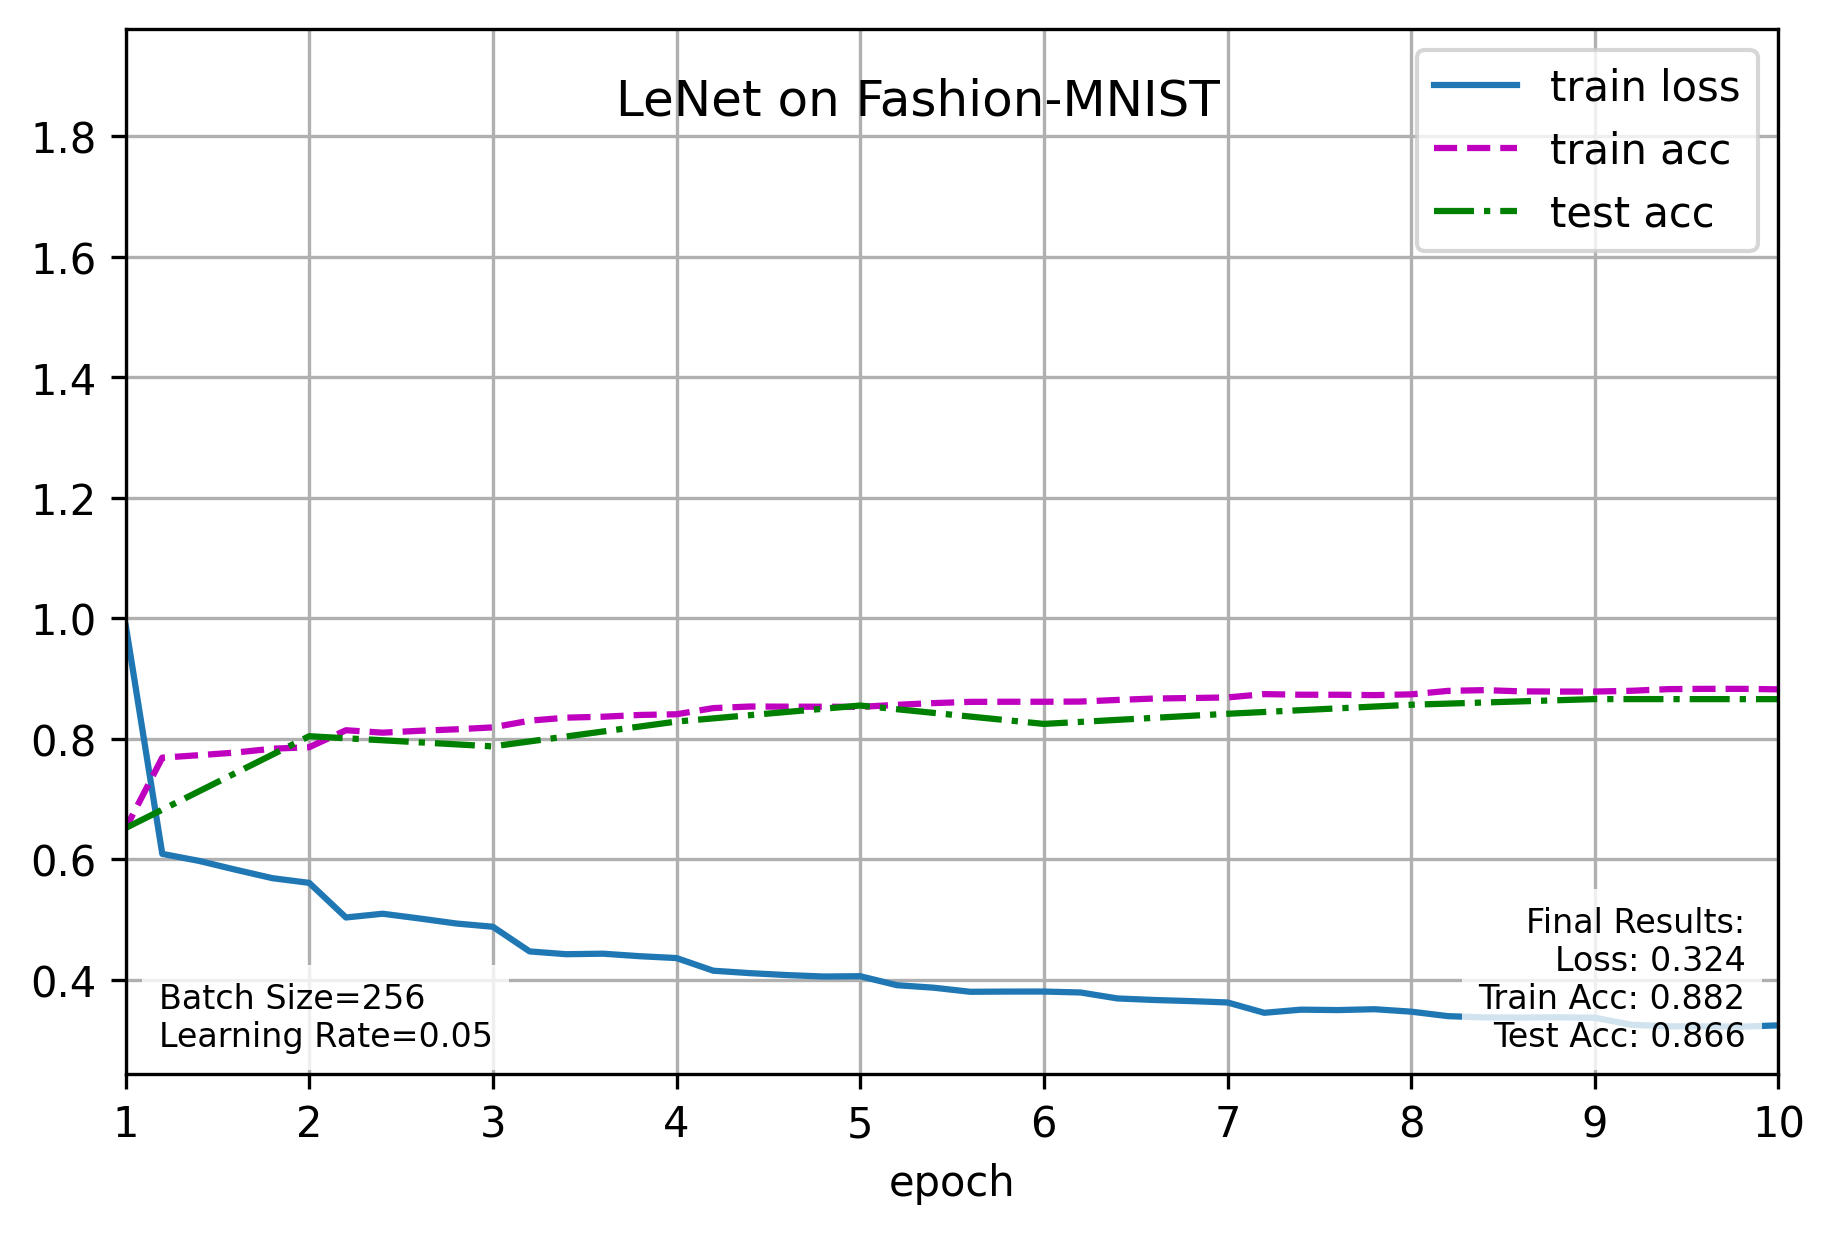
\includegraphics[width=0.6\textwidth]{picture/lenet_on_fashion-mnist_bs256_lr0.05_20241110_221637.png}
    \caption{LeNet 使用 0.05 学习率训练结果}
\end{figure}
\vfill  % 自动分配垂直空间

\begin{figure}[H]
    \centering
    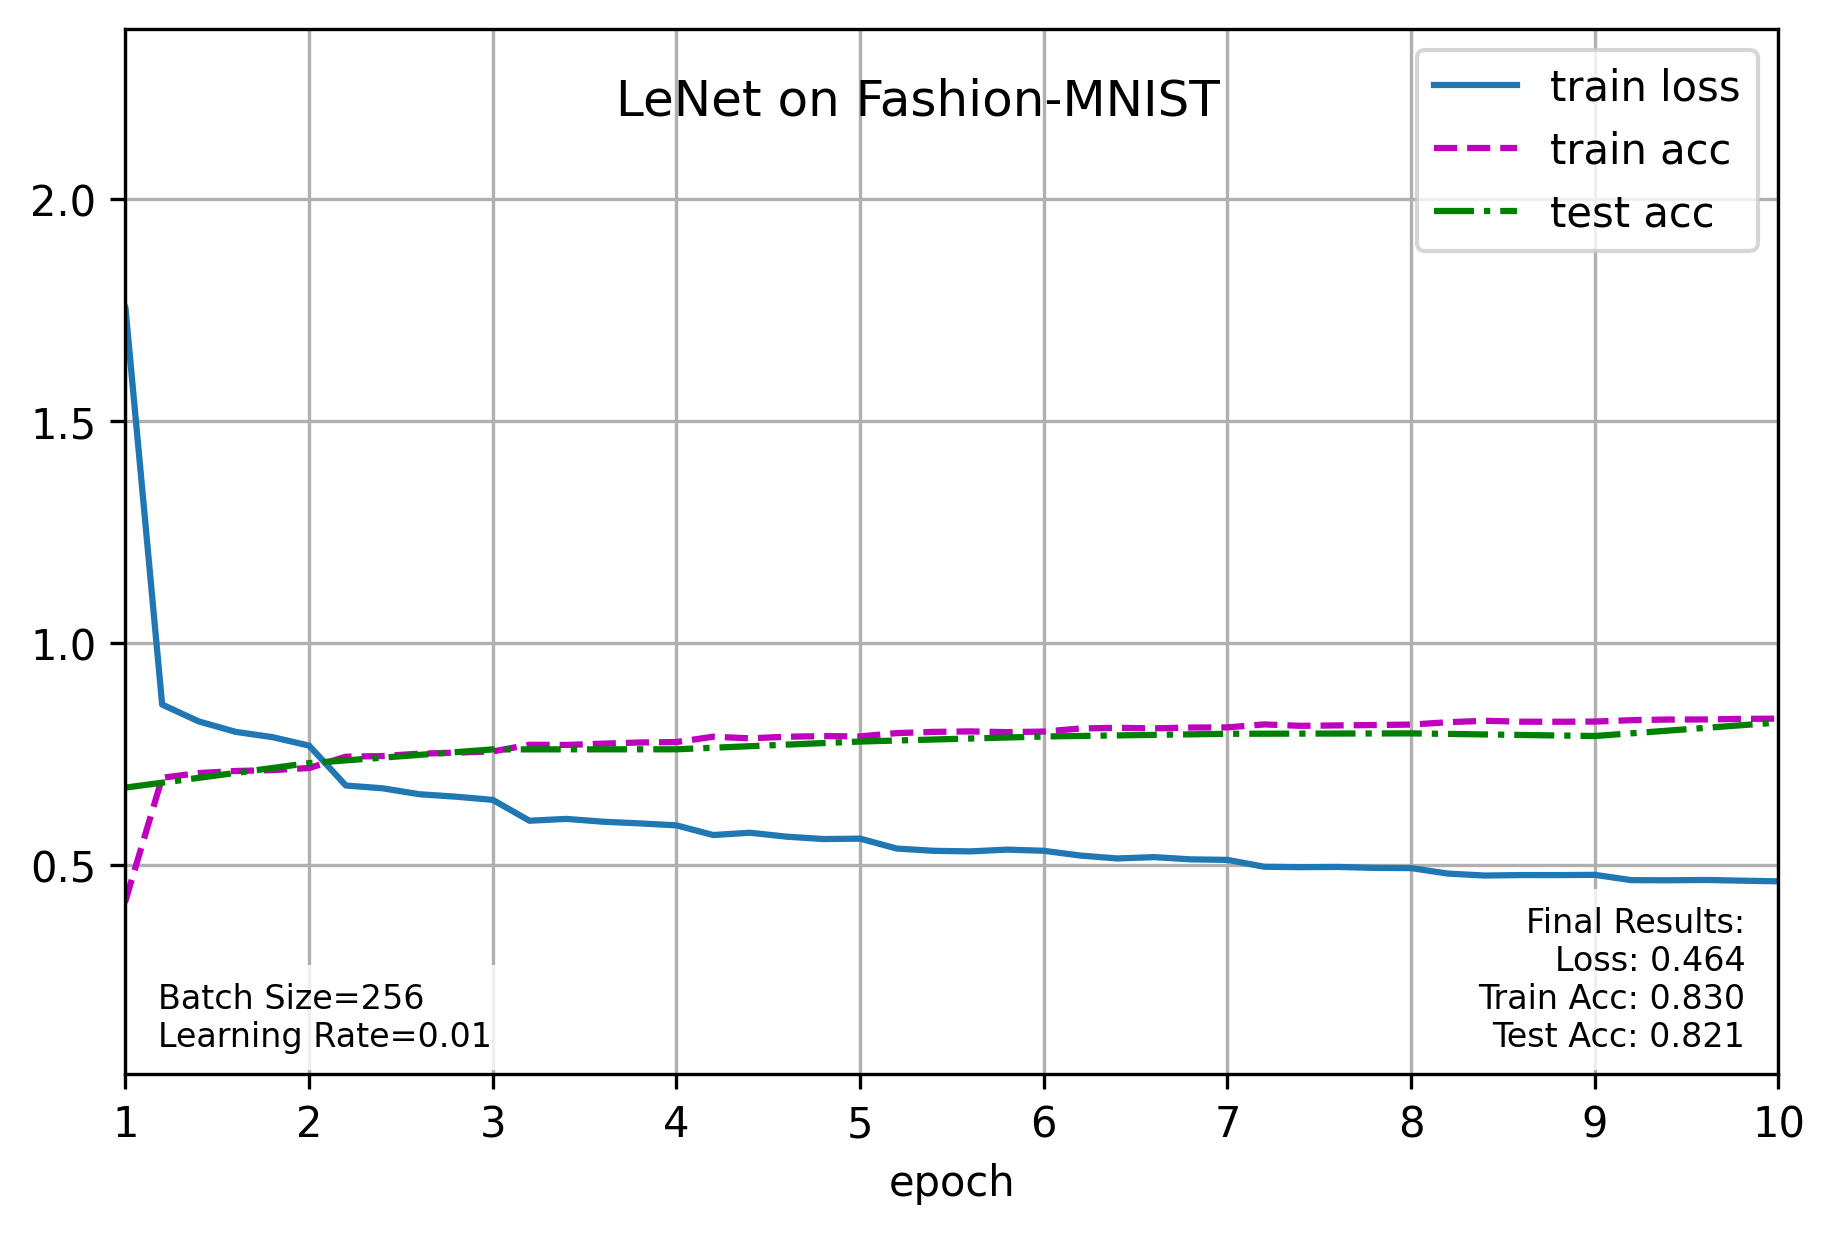
\includegraphics[width=0.6\textwidth]{picture/lenet_on_fashion-mnist_bs256_lr0.01_20241110_222304.png}
    \caption{LeNet 使用 0.01 学习率训练结果}
\end{figure}
\end{minipage}
\end{center}

\newpage
\subsection{ResNet18 在不同学习率下的训练结果}
\begin{center}
\begin{minipage}{\textwidth}
\begin{figure}[H]
    \centering
    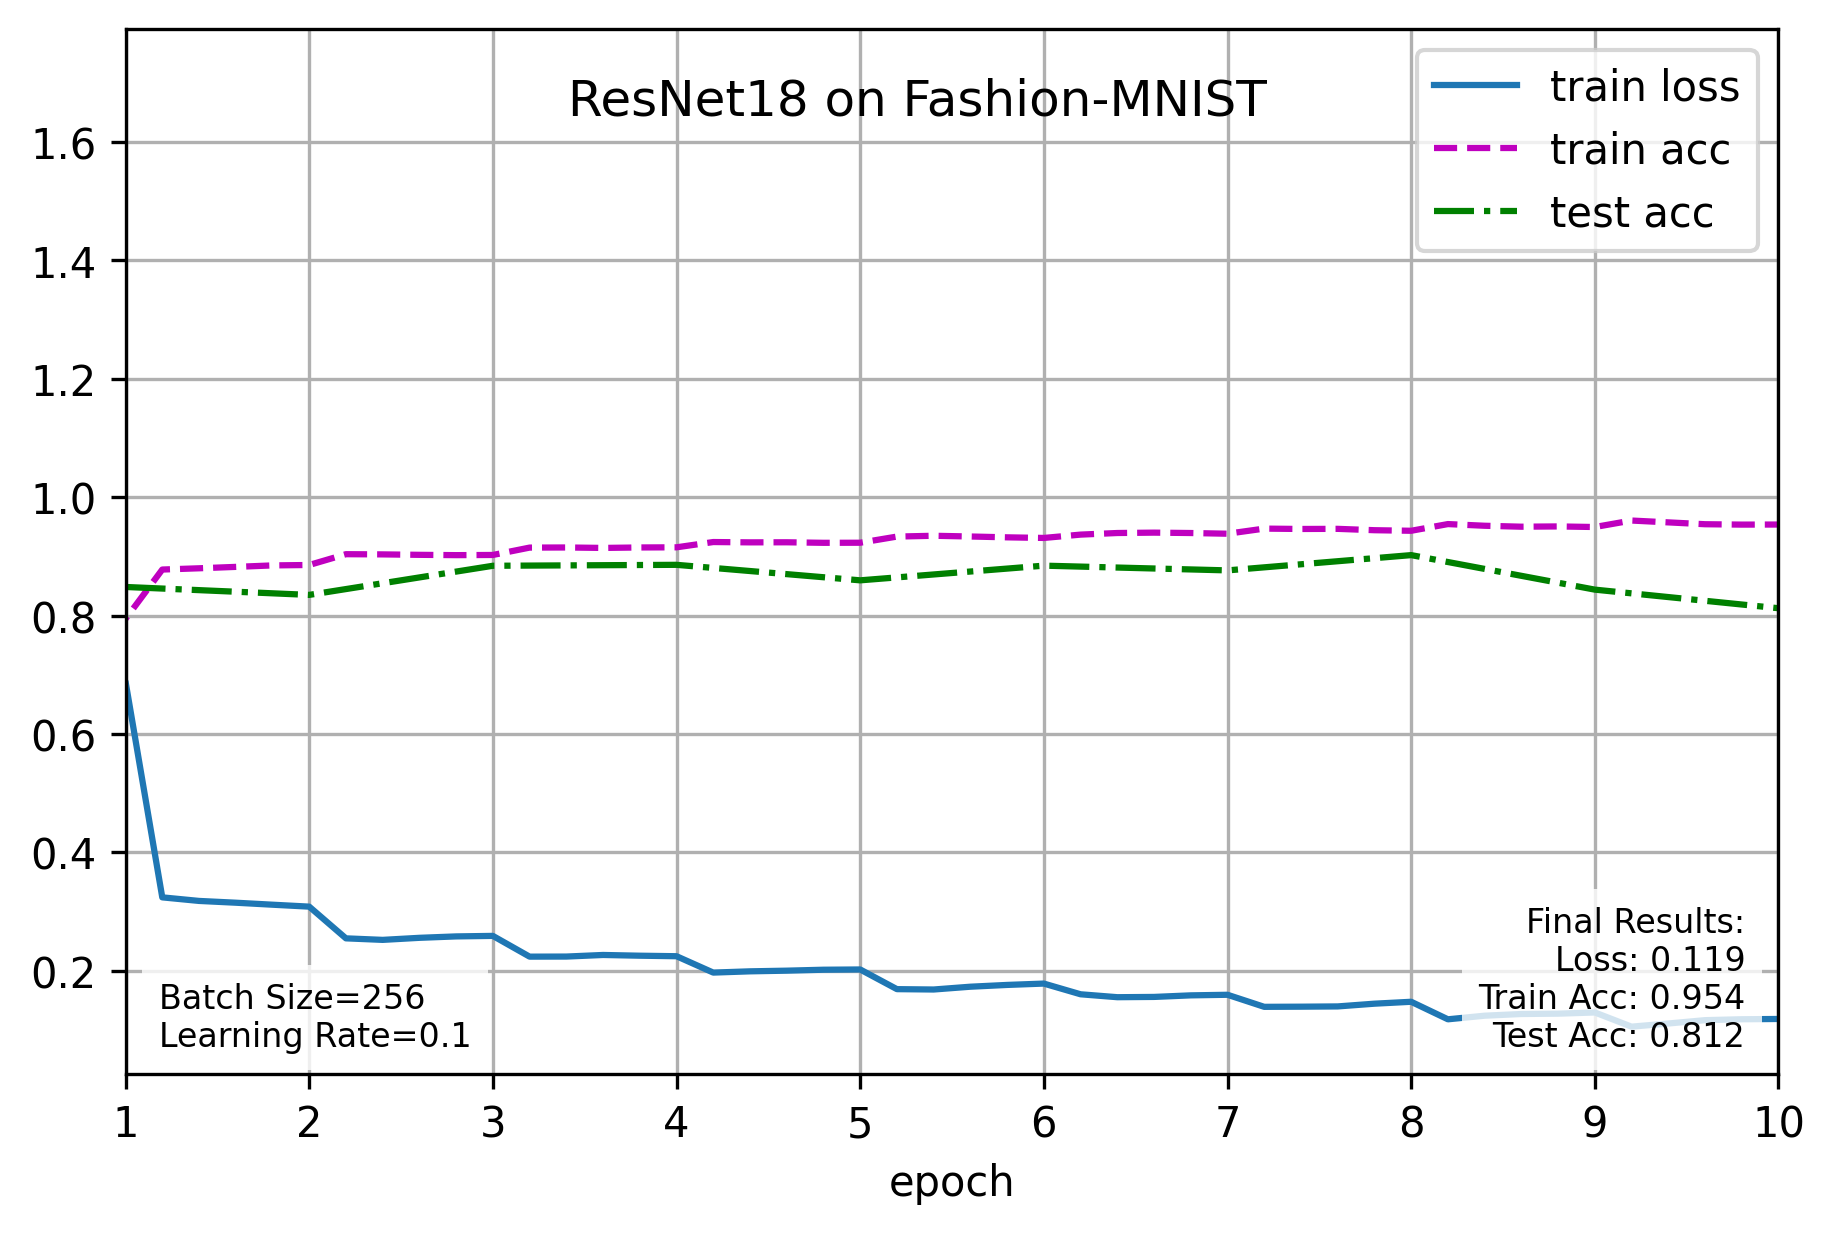
\includegraphics[width=0.6\textwidth]{picture/resnet18_on_fashion-mnist_bs256_lr0.1_20241110_221226.png}
    \caption{ResNet18 使用 0.1 学习率训练结果}
\end{figure}
\vfill

\begin{figure}[H]
    \centering
    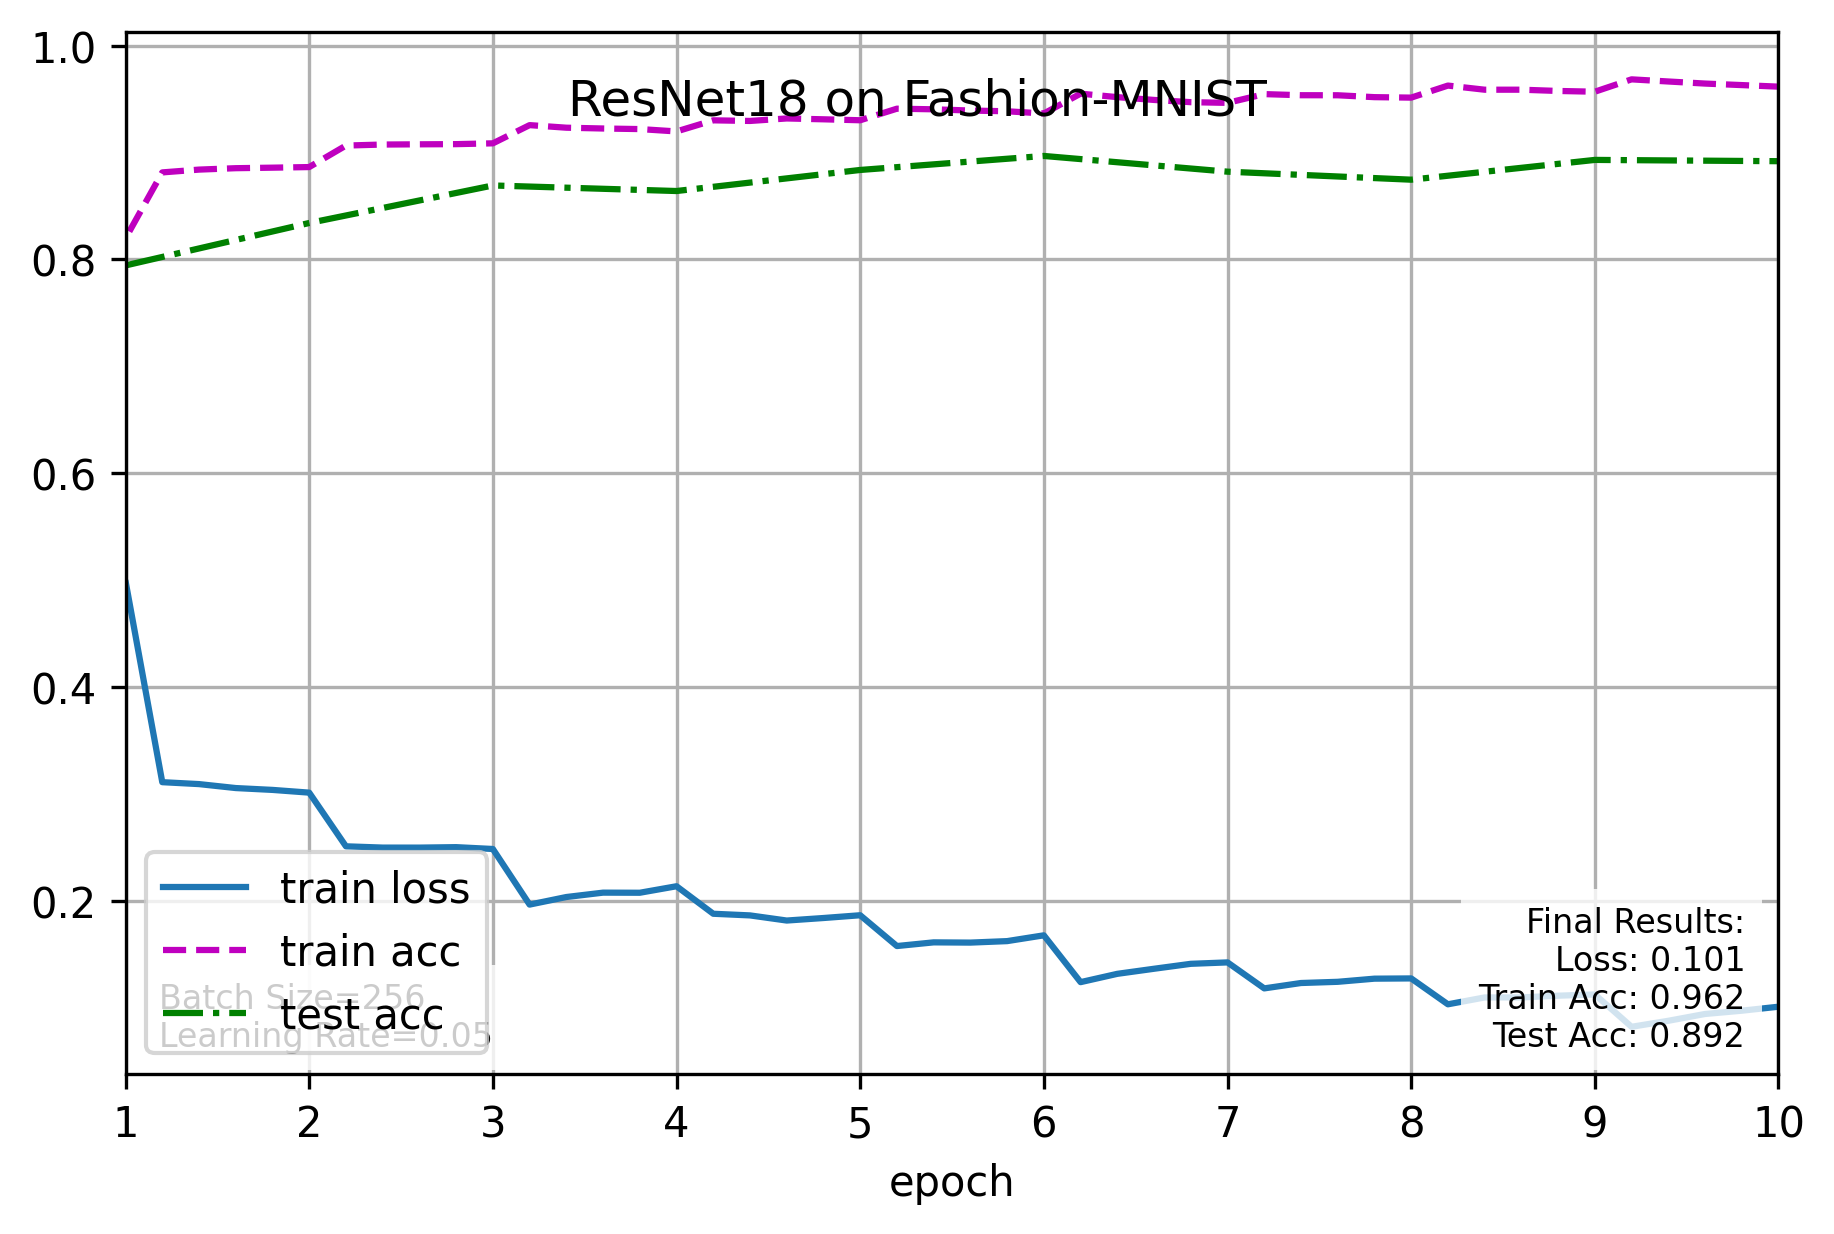
\includegraphics[width=0.6\textwidth]{picture/resnet18_on_fashion-mnist_bs256_lr0.05_20241110_221842.png}
    \caption{ResNet18 使用 0.05 学习率训练结果}
\end{figure}
\vfill

\begin{figure}[H]
    \centering
    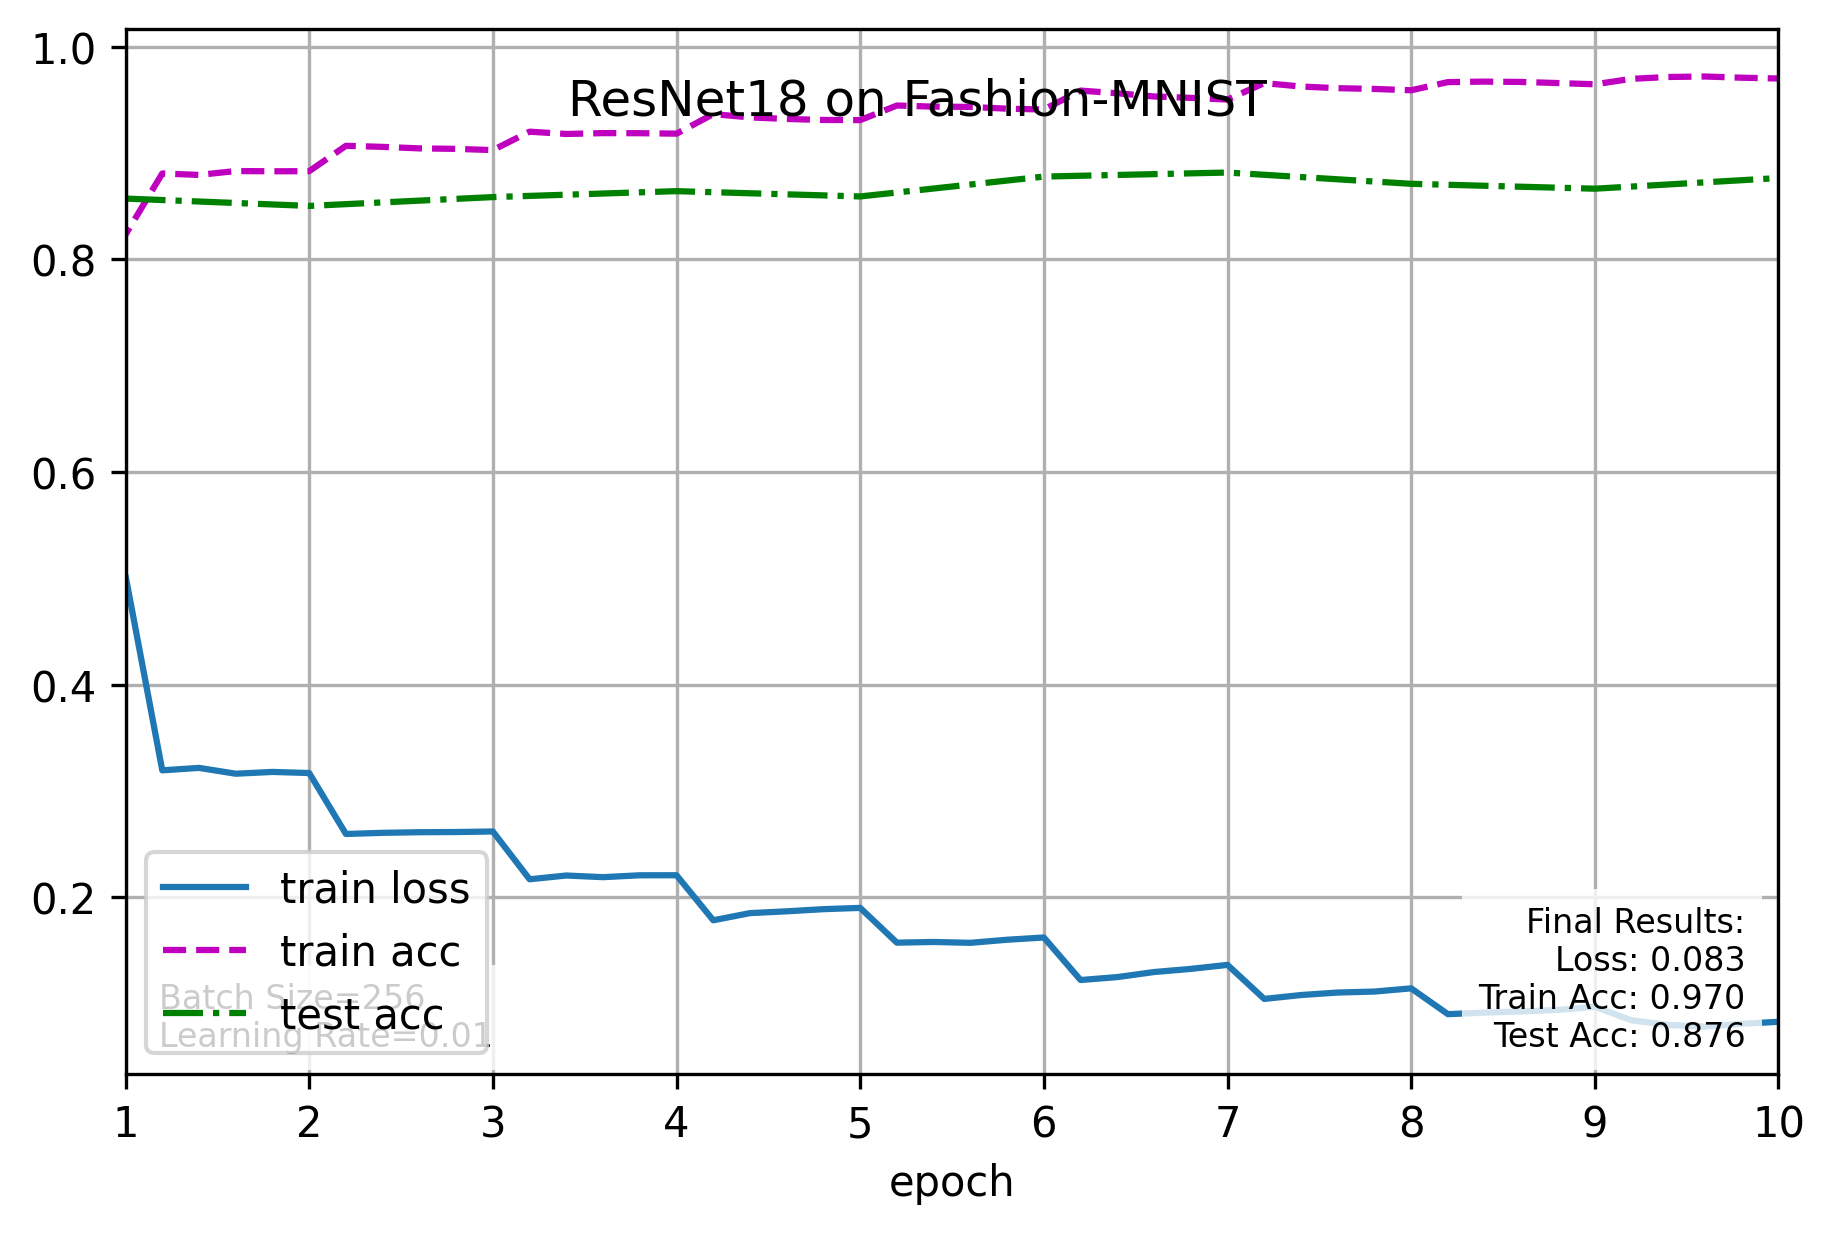
\includegraphics[width=0.6\textwidth]{picture/resnet18_on_fashion-mnist_bs256_lr0.01_20241110_222516.png}
    \caption{ResNet18 使用 0.01 学习率训练结果}
\end{figure}
\end{minipage}
\end{center}

\newpage
\subsection{ResNet34 在不同学习率下的训练结果}
\begin{center}
\begin{minipage}{\textwidth}
\begin{figure}[H]
    \centering
    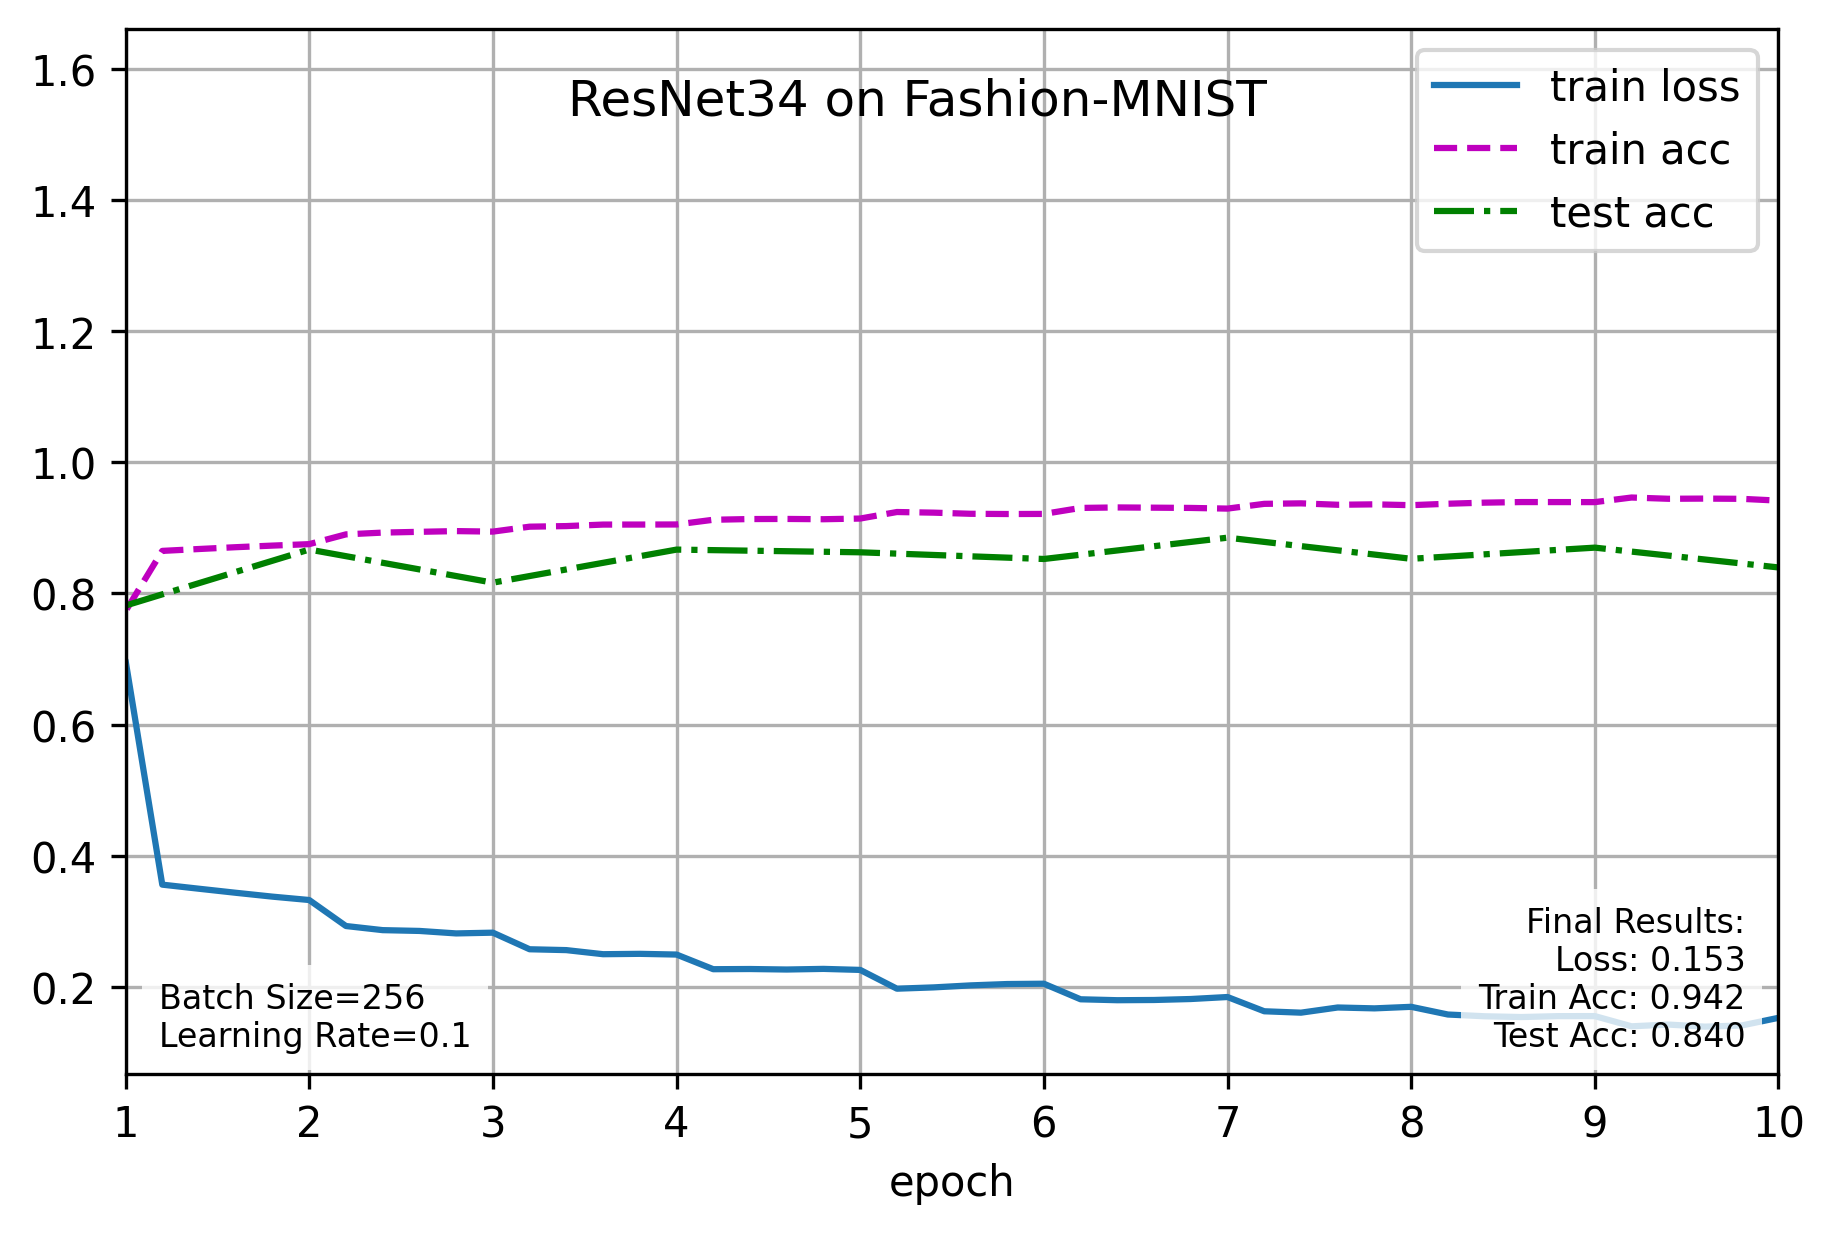
\includegraphics[width=0.6\textwidth]{picture/resnet34_on_fashion-mnist_bs256_lr0.1_20241110_221450.png}
    \caption{ResNet34 使用 0.1 学习率训练结果}
\end{figure}
\vfill

\begin{figure}[H]
    \centering
    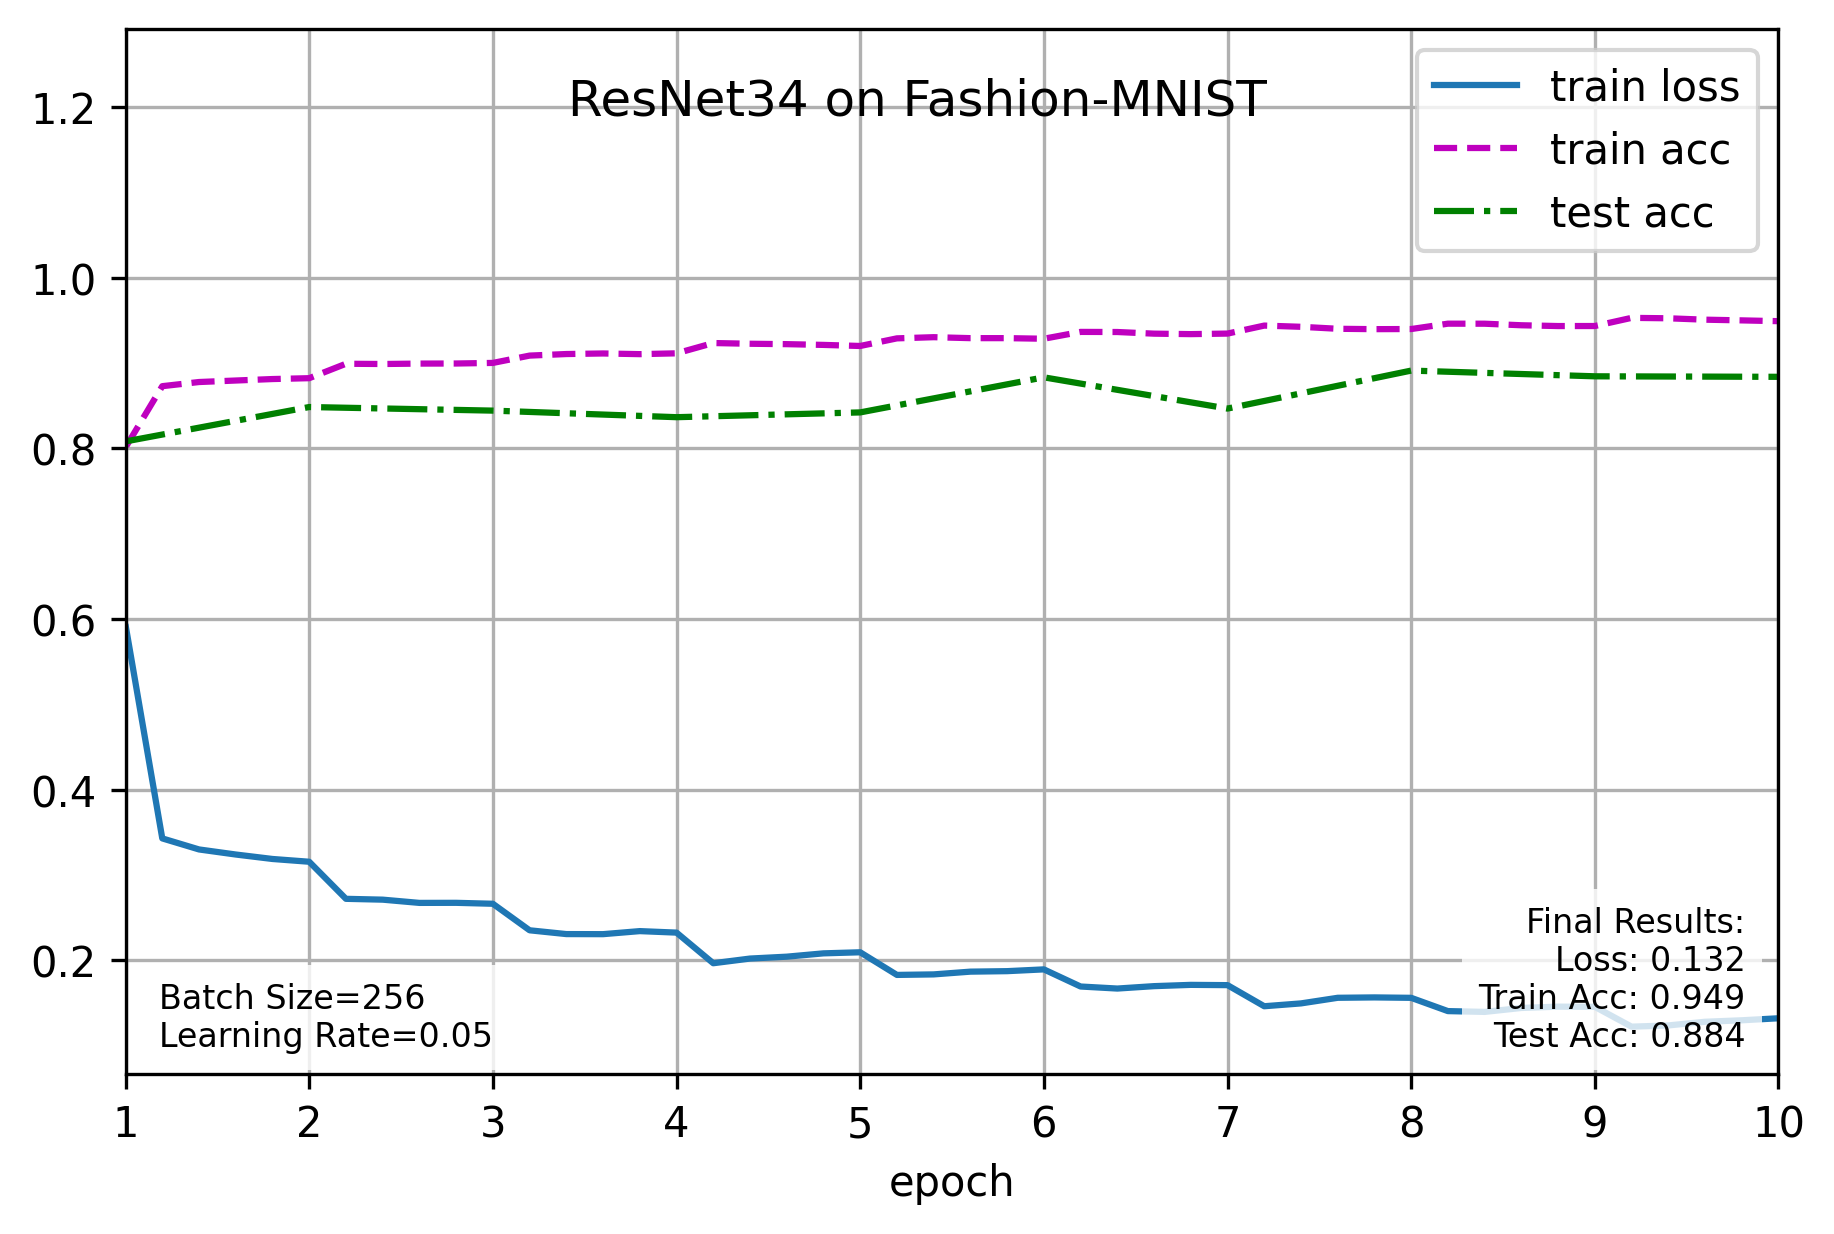
\includegraphics[width=0.6\textwidth]{picture/resnet34_on_fashion-mnist_bs256_lr0.05_20241110_222110.png}
    \caption{ResNet34 使用 0.05 学习率训练结果}
\end{figure}
\vfill

\begin{figure}[H]
    \centering
    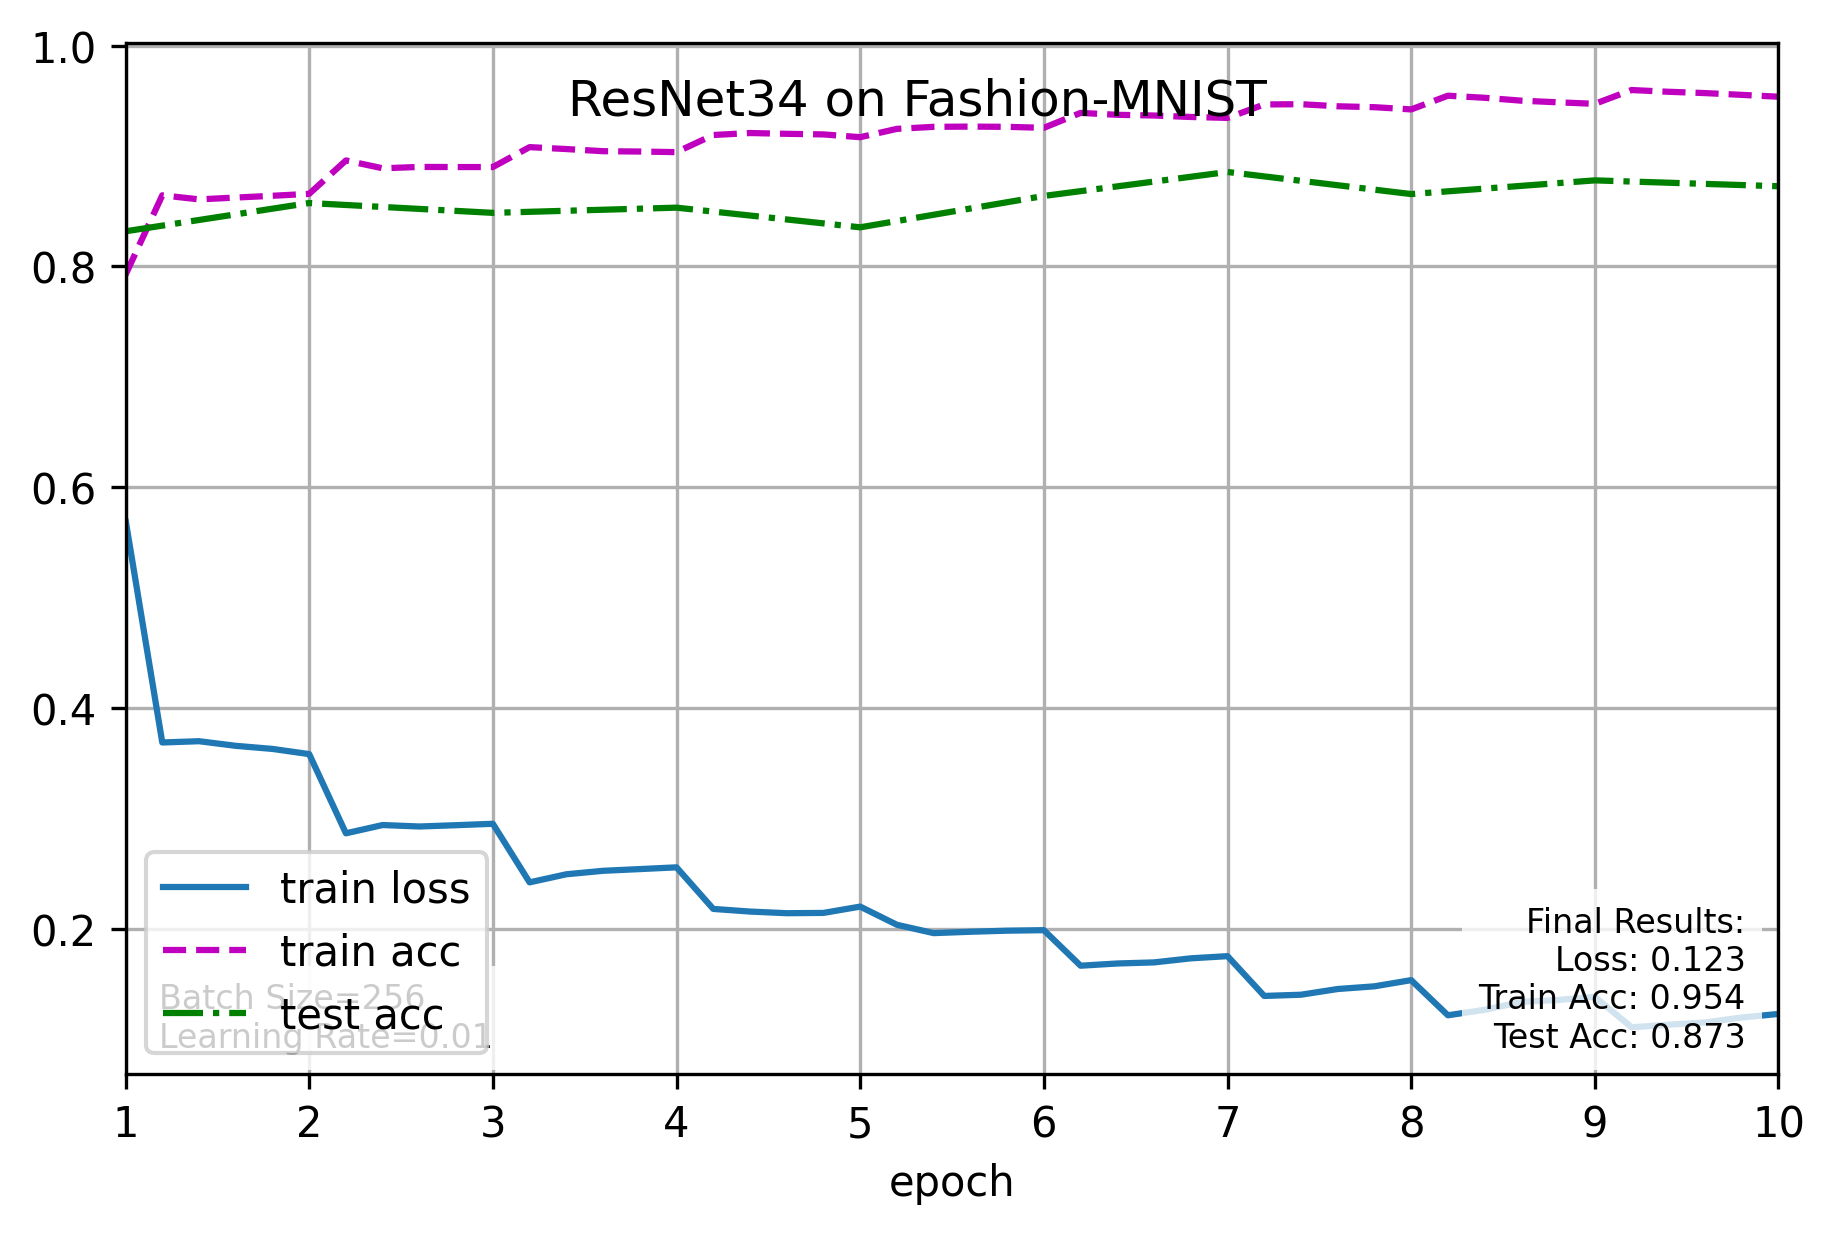
\includegraphics[width=0.6\textwidth]{picture/resnet34_on_fashion-mnist_bs256_lr0.01_20241110_222753.png}
    \caption{ResNet34 使用 0.01 学习率训练结果}
\end{figure}
\end{minipage}
\end{center}


\newpage
\section{附录:关键代码示例}
\subsection{LeNet 模型定义}
\begin{lstlisting}[language=Python]
class LeNet(nn.Module):
    """LeNet-5卷积神经网络架构"""
    def __init__(self):
        super().__init__()
        self.conv = nn.Sequential(
            # 第一个卷积层 (1, 28, 28) -> (6, 24, 24)
            nn.Conv2d(1, 6, kernel_size=5, padding=0),
            nn.ReLU(),
            # 第一个池化层 (6, 24, 24) -> (6, 12, 12)
            nn.MaxPool2d(kernel_size=2, stride=2),
            # 第二个卷积层 (6, 12, 12) -> (16, 8, 8)
            nn.Conv2d(6, 16, kernel_size=5),
            nn.ReLU(),
            # 第二个池化层 (16, 8, 8) -> (16, 4, 4)
            nn.MaxPool2d(kernel_size=2, stride=2)
        )
        
        self.fc = nn.Sequential(
            nn.Flatten(),
            nn.Linear(16 * 4 * 4, 120),
            nn.ReLU(),
            nn.Linear(120, 84),
            nn.ReLU(),
            nn.Linear(84, 10)
        )
\end{lstlisting}

\subsection{ResNet的残差块实现}
\begin{lstlisting}[language=Python]
class ResidualBlock(nn.Module):
    """ResNet的基本残差块
    
    这是ResNet中的基本构建块,包含两个3x3卷积层和一个shortcut连接。
    如果输入和输出维度不匹配,会通过1x1卷积进行调整。
    
    Args:
        in_channels (int): 输入通道数
        out_channels (int): 输出通道数 
        stride (int): 步长,用于下采样,默认为1
    """
    expansion = 1  # 输出通道数相对于输入通道数的倍增系数
    def __init__(self, in_channels, out_channels, stride=1):
        super().__init__()
        # 第一个卷积层: 3x3卷积,可能改变特征图大小和通道数
        self.conv1 = nn.Conv2d(in_channels, out_channels, kernel_size=3, 
                              stride=stride, padding=1, bias=False)
        self.bn1 = nn.BatchNorm2d(out_channels)  # 批量归一化层
        # 第二个卷积层: 3x3卷积,保持特征图大小和通道数不变
        self.conv2 = nn.Conv2d(out_channels, out_channels, kernel_size=3,
                              padding=1, bias=False)
        self.bn2 = nn.BatchNorm2d(out_channels)  # 批量归一化层
        # shortcut连接: 用于将输入直接加到输出上
        self.shortcut = nn.Sequential()  # 默认为恒等映射
        # 当步长不为1或通道数改变时,需要调整shortcut分支的维度
        if stride != 1 or in_channels != out_channels:
            self.shortcut = nn.Sequential(
                # 1x1卷积用于调整维度
                nn.Conv2d(in_channels, out_channels, kernel_size=1,
                         stride=stride, bias=False),
                nn.BatchNorm2d(out_channels)
            )
    def forward(self, x):
        identity = x  # 保存原始输入用于shortcut连接
        # 第一个卷积块: 卷积+BN+ReLU
        out = torch.relu(self.bn1(self.conv1(x)))
        # 第二个卷积块: 卷积+BN(注意这里没有ReLU)
        out = self.bn2(self.conv2(out))
        # 残差连接: 将shortcut分支的结果加到主分支上
        out += self.shortcut(identity)
        return torch.relu(out)  # 最后再通过ReLU激活
\end{lstlisting}

\subsection{数据集加载与预处理}
\begin{lstlisting}[language=Python]
        # 获取数据集的均值和标准差
        mean, std = self._get_mean_std()

        self.transform = transforms.Compose([
            transforms.ToTensor(),  # 将图像转换为张量
            transforms.Normalize(mean, std)  # 进行标准化
        ])
\end{lstlisting}

\subsection{训练代码}
\begin{lstlisting}[language=Python]
def train(net, train_iter, test_iter, num_epochs, lr, device, title=None):
    """训练模型的主函数
    
    Args:
        net: 要训练的神经网络模型
        train_iter: 训练数据集迭代器
        test_iter: 测试数据集迭代器 
        num_epochs: 训练轮数
        lr: 学习率
        device: 训练设备(CPU/GPU)
        title: 图表标题,默认使用模型类名
    """
    net.to(device)  # 将模型移至指定设备
    # 定义优化器和损失函数
    optimizer = torch.optim.SGD(net.parameters(), lr=lr)
    loss = nn.CrossEntropyLoss()
    timer, num_batches = Timer(), len(train_iter)
    for epoch in range(num_epochs):
        # 训练损失之和,训练准确率之和,样本数
        metric = Accumulator(3)
        net.train()  # 设置为训练模式
        for i, (X, y) in enumerate(train_iter):
            timer.start()
            optimizer.zero_grad()  # 清除梯度
            X, y = X.to(device), y.to(device)
            y_hat = net(X)
            l = loss(y_hat, y)
            l.backward()
            optimizer.step()
            with torch.no_grad():
                metric.add(l * X.shape[0], accuracy(y_hat, y), X.shape[0])
            timer.stop()
            # 计算当前批次的训练损失和准确率
            train_l = metric[0] / metric[2]
            train_acc = metric[1] / metric[2]
        test_acc = evaluate_accuracy_gpu(net, test_iter)
        animator.add(epoch + 1, (None, None, test_acc))
    print(f'loss {train_l:.3f}, train acc {train_acc:.3f}, '
          f'test acc {test_acc:.3f}')
    print(f'{metric[2] * num_epochs / timer.sum():.1f} examples/sec '
\end{lstlisting}

\end{document}